\documentclass[12pt,a4paper]{article}
\usepackage[hang,small,bf]{caption}
\usepackage[strict]{changepage}
\usepackage[top=2.5cm,right=2.5cm,bottom=2.5cm,left=2.5cm]{geometry}
\usepackage{graphicx}
%\usepackage[pdfborderstyle={/S/U/W 1}]{hyperref}
\usepackage{ifpdf}
\usepackage{moreverb}
\usepackage{url}
\usepackage[utf8]{inputenc}
\usepackage[UKenglish]{babel}
\ifpdf
\pdfinfo {
	/Author (Tommy Anh Tuan Nguyen)
	/Title ()
	/Subject ()
	/Keywords (artificial intelligence, benchmarks, c++, computational development, framework, genetic algorithm, memory, optimization, performance, speed)
	/CreationDate (D:20080909223146)
}
\fi
\def\verbatimtabsize{4\relax}
\graphicspath{{./graphics/}}
\setlength\fboxsep{0pt}
\setlength\fboxrule{0.5pt}
\begin{document}
	\begin{titlepage}
		\changepage{}{}{2cm}{2cm}{}{3cm}{}{}{}
		\large\noindent
		Tommy Anh Tuan Nguyen\newline\newline\newline
		\includegraphics[scale=0.4]{../ngene_logo}\newline
		{\LARGE An Artificial Development Framework}\newline
		\newline
		\newline
		\newline
		\newline
		\newline
		\newline
		Trondheim, December 2008\newline
		\newline
		\newline
		{\Large Norwegian University of Science and Technology}\newline
		Faculty of Information Technology, Mathematics\newline
		and Electrical Engineering\newline
		Department of Computer Science (IDI)\newline
		\newline
		\newline
		Master's Thesis in Computer Science, Artificial Intelligence\newline
		\newline
		Supervised by Pauline Haddow, IDI
	\end{titlepage}
	\begin{abstract}
	Nyuu...
	\end{abstract}
	\newpage
	\noindent\textbf{\large Acknowledgements}\newline
	My deepest gratitude goes to my supervisor for her seemingly infinite wisdom and patience, and my parents for their unconditional love and support. I would also like to thank my friends for the days I didn't feel like working, and my girlfriend for being so patient with me.\newline
	\newline
	Last but not least, Haruhi and Chii, without whom this thesis would be nigh impossible.
	\newpage
	\pagestyle{headings}
	\tableofcontents
	\listoffigures
	\newpage
	\section{Introduction}
Humans have always been limited in their capacity and knowledge. There are problems that we cannot solve by brain power alone. The first computers came therefore into existence, made to do tasks that we found too heavy, tedious or even difficult. Today, this has become more of a reliance than ever. Computers has not only become ridiculously faster but are also practically everywhere. Whether we like it or not, it has become essential for a modern society.

However, the problem with computers, just like it was aeons ago, is that it still needs to be told what to do. If a problem is too difficult for us to describe precisely, it cannot solve it. Even if we do manage to program it to solve a very difficult problem, it may use too much resources. Sometimes, it is better to get an estimation of the answer. A genetic algorithm is a search method that has this ability. It may not find optimal results but more often than not, the results are sufficiently satisfactory for given problem. This comes in handy when thorough search is too costly or not possible.

While this method has been applied in many applications already, there are still aspects of it that need to be addressed. One major concern is that of scalability. The most common way to map a genotype to phenotype, as it was back in the beginning, is often directly. An alteration in a single trait in the genotype had a direct effect on traits in the phenotype. For small applications, this method is sufficiently efficient. However, as problems increase in size and complexity, the genotype too will grow larger and more complex. Eventually, it will become computationally infeasible as well.

Since genetic algorithms are inspired by natural selection, it is only obvious that possible solutions to the scalability problem could also stem from biology. If we look at how some organisms came to be, we know that most of these start out as a single cell. The cell divides and become two cells. These cells divides once more two become four, and this process is kept going until it reaches maturity. The whole process is coordinated with the help of the DNA and some interactions. This is nature's way to tackle the scalability problem. Drawing inspiration from genome and cellular activities, many development models have been created. Whether they make use of a DNA or applies a different approach, they all inherit the idea of a single entity, duplicating itself until a whole organism is grown to a satisfactory size and shape. As it turns out, it was difficult to learn from these models. It was hard to determine what worked, or didn't. It seemed that every model had its own quirks, showing that some properties are beneficial while others claimed the opposite. How do we then know what is right and what is wrong? What factors had an effect on the models? How do we know it is not the model that is at fault but a smaller detail somewhere else?

This thesis does not seek to answer such questions. Instead, it wishes to make them disappear by introducing a common platform on which models can be implemented. If all models utilized a common platform, many trivial factors will disappear simply because of the fact that any model implemented within this framework will use the same implementation for anything that is common in artificial development, save the model itself. As the thesis goes on, this will hopefully become much clearer. By providing a common ground, the focus will shift away from the underlying structure, to the models themselves. The requirements of such a framework will come to light in the following chapters.

\subsection{Biological Development}
Biological development is a term used to describe the process where organisms grow and develop. In humans, for example, the process in which a fertilized egg grows and develops into a fetus is an area that is studied in biological development. This process can be applied to computer science but instead of organisms, it may be a picture, a solution to a problem, or even software to control a robot.

The following listing is compiled words, and their meaning, that are commonly used when discussing artificial development in general and particularly in this thesis.

\begin{itemize}
\itemsep=0pt
	\item\textbf{ADCGP} or artificial development is the shorter name for \emph{artificial development using Cartesian genetic programming}. Method and model invented by Dr. Julian F. Miller. A cell program based model.
	\item\textbf{ArtDev3D} is the other model discussed in this thesis. Written by Johan H{\o}ye for his master's thesis. A DNA based model.
	\item\textbf{Cell program} is the program of a cell. However, it is loosely used as a term for all the cellular activities that take place in a development step when talking about the framework.
	\item\textbf{Artificial/computational development} are the terms used to describe biological development applied to computers.
	\item\textbf{Development step} or \textbf{tick} is a single unit of growth. With each step, cells partake in activities that contribute to the growth of an organism.
	\item\textbf{Evolutionary algorithm} is a search method inspired by biology and applies concepts of reproduction, mutation and selection to computers.
	\item\textbf{Genetic algorithm} is a class of evolutionary algorithms that are often used to solve optimization problems
	\item\textbf{Genetic programming} is another class of evolutionary algorithms. This technique is applied when trying to find an algorithm that is able to solve some predefined tasks.
	\item\textbf{Genotype} is the genetics of an organism. It is the ``recipe'' for an organism.
	\item\textbf{Organism} refers to the entity that contains a genotype and cells. The state of an organism starts out with a single cell to ``fully'' grown.
	\item\textbf{Phenotype} is the end result of a genotype. It is the resultant organism that we see when it is fully grown.
\end{itemize}

\subsection{Motivation}
While evolutionary computation has been around for a while, artificial development is still at an early stage. There is still a lot to study in this field. Though researchers have already made great progress in this field, there are things that aren't quite figured out yet. When ArtDev3D was presented two years ago, it created a controversy because it showed that chemicals weren't all that beneficial to development. This was direct contradiction to other articles in the field. For a couple of years already, chemicals have shown to be beneficial when working with artificial development. However, it was then later discovered that chemicals were used differently in these models. While chemicals were used to exchange information between cells, ArtDev3D only used it internally to activate proteins. There may also have been other factors that affected this outcome, though it was fairly difficult to determine. This only raised more questions than there were answers for. Of course, more thorough studies could have been done but these models were built on different platforms as well. Any study of these would have to take into account too many factors to give reliable results.

One may then ask if there isn't anything that can be done to make these uncertainties go away. First of all, it is nearly impossible to remove any uncertainty, as this will always be present to some extent. However, it is entirely possible to reduce the number of factors such that the equation balances out. This can be achieved by introducing a common ground that every model will share except for what makes it unique. Just like how an operating system provides all the necessary infrastructure so that different softwares can be useful to us, a similar platform should also exist to provide any development model what is needed. Such a platform will not eliminate factors but make the factors not matter because they are the same for all models. All cells will have the same definition in all models. All models will use the same development algorithm. The focus shift to the models will clearly show what the differences are, hopefully making studies of this nature even more fruitful than it has been thus far.

\subsection{Where do we go from here?}
In the following chapter, we will have a look at the two models that have been chosen for this project. We will look at the idea behind them and see how they work. We will also discuss their differences and explain why a framework is necessary. We will also be looking at requirements for such a framework. In chapter~\ref{sec:implementation}, we shall take a look at the implementation of the framework and the porting of mentioned models over to the framework. This section will describe the most important details that is relevant to their re-implementation. Any changes made during this process will be highlighted and explained. With chapter~\ref{sec:experiments}, it will be shown that it is possible to reproduce the results gotten in past experiments. Some experiments will be picked out and tested on the new implementations of two models. The results are then compared and discussed. This is a necessary step in order to prove that it is in fact possible to implement different models within the framework.

	\section{Development Models}
There are many development models in the field that are inspired by nature. Though the concept of biological development does not change much, it is very much still a topic under discussion and there are still uncharted territories. It is therefore not surprising that these models differ not only in implementation, but also the biological ideas behind it. In this chapter, we will take a look at two models. We'll see how they work, and discuss their differences. These models are important for this thesis because they are believed to represent the greatest difference in development models to date.

\subsection{ArtDev3D}
\label{sec:Models:ArtDev3D}
In 2006, Johan H{\o}ye handed in his master's thesis\cite{hoye2006} based on his own model of biological development. Its aim was to draw inspiration from biology but simplify concepts to avoid dwelling too deep into the underlying and less understood concepts.

\subsubsection{Concepts}
To understand this model, we will have to touch a few topics in biology. Like with humans, everything starts out with a single cell, the zygote. The zygote divides and becomes two cells. These cells divide again to become four cells. This process repeats itself in a controlled fashion with the help of the DNA, the recipe of life. It tells which proteins to synthesize, how and when. The proteins, in turn, carry out all the actual work inside the cell. In his model, only four such tasks were defined:

\begin{itemize}
	\itemsep=0pt
	\item Change the type of the cell
	\item Regulate chemical levels
	\item ``Request'' cell division in several directions
	\item Synthesize/transcribe more proteins
\end{itemize}

I use ``request'' here because of the way this model works. The proteins queue a request for the cell to perform division in some directions. These requests are accumulated and if the stimuli levels are just right, it will be realized. Likewise, the proteins also request for a change of cell type. The proteins themselves need to be activated in order to request anything. This usually depends on the current chemical levels in the cell as well as nearby cells. The neighbourhood in this model is defined to be the cells that a cell are in direct contact with in free space. That is above, below, left, right, front and back. Six in total.

The cell is also ``programmed'' to perform a number of tasks independent of the DNA. Implemented functions include osmosis, or the exchange of chemicals (or hormones) with nearby cells, and performing the actual cell division in requested directions. This set of functions are fixed for every cell and is not changed through evolution like the DNA is.

\begin{figure}[!ht]
	\centering
	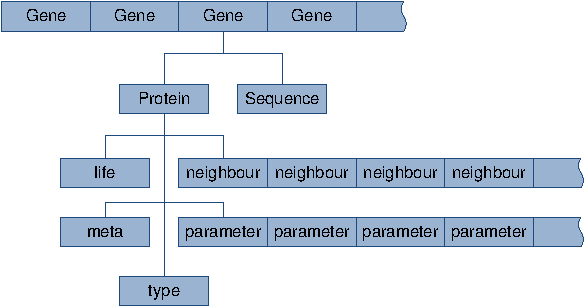
\includegraphics[scale=1.2]{artdev3d_genotype}
	\caption{Genotype representation in ArtDev3D}
	\label{fig:artdev3d_genotype}
\end{figure}

The genotype of this model (see fig~\ref{fig:artdev3d_genotype}), the DNA, is an array with genes. The genes carry a recipe for a protein and a genetic sequence. The gene sequence is used to find genes with desired proteins to synthesize. The protein type determines what its function is. If a protein that changes the cell's type is a type, then proteins that regulate chemicals are another. When the protein is activate is stored in the neighbours and chemicals array. The neighbours array stores the desired types of nearby cells. The chemicals array stores the desired chemical levels in the cell. When both of these are fulfilled, the protein is activated. Data in \texttt{meta} contain only one of two things, a cell type or a genetic sequence. These are used by the cell-type-changing and transcribing proteins respectively. The other two types only use the parameters. Figure~\ref{fig:artdev3d_protein-parameters} shows how the parameters are used to store the values to adjust the chemicals in a cell. Likewise, the proteins can store the directions it wants cells to divide into.

\begin{figure}[!ht]
	\centering
	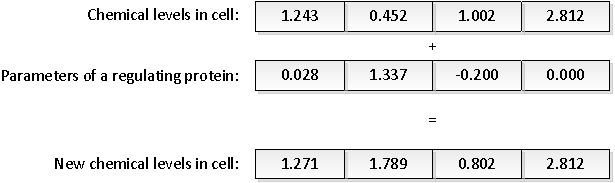
\includegraphics[scale=1.2]{artdev3d_protein-parameters}
	\caption{Parameters representation in ArtDev3D}
	\label{fig:artdev3d_protein-parameters}
\end{figure}

Any of these properties can be easily mutated and still be duplicated as a whole during cross over.

\subsubsection{How it works}
Development starts with an ``empty'' organism. The DNA is inserted into a cell before it is inserted to the organism. It becomes a zygote once the cell ``scans'' through the DNA and synthesizes all proteins. This is only performed in the initial cell. After initialization, the organism is developed by performing a set of operations on every cell every development step:

\begin{enumerate}
	\itemsep=0pt
	\item Determine activated proteins, usually by checking the internal chemical levels and neighbour cell types.
	\item All activated proteins request an action.
	\item Actions are accumulated, and executed. Depending on the action, the cell may regulate its chemical levels, synthesize proteins, change type, and perform cell division.
\end{enumerate}

Note that while the DNA indirectly requests actions upon the cell through the proteins, the cell performs the real work, like regulating the chemicals and proteins, behind the scene. The cell functions limit what the DNA can do, but at the same time, the DNA can affect both the cell and its surroundings using proteins as its proxy.

The development ends when a number of steps have passed, and the organism is rated based on how similar it is to the target phenotype. In this case, the targets are usually simple three-dimensional shapes.

While working with this model, it was discovered that the development algorithm does not develop all cells simultaneously. Usually, all cells must receive or gather information on nearby cells before any actions are executed. This is not the case here. Every cell gathers information and executes action in one go. So when the next cell gathers information, there will be ``new'' information mixed in. This flow is described in more detail in chapter~\ref{sec:Implementation:ArtDev3D}. However, the model seem to work rather well regardless. H{\o}ye's experiments also showed a number of interesting things. The initial number of don't-care-neighbours, i.e.\ the number of neighbours that can be of any type, had a negative impact on the growth of an organism when lowered. It was also shown that having a higher number of chemical types in the cells only contributed to making it harder to correctly develop the target shapes. This is most interesting because the next model we are going to discuss is based on chemicals, and it has been shown to work well.


\subsection{Artificial Development (ADCGP)}
Artificial development using Cartesian genetic programming is built on a genetic program invented by Julian Miller in 1998. The following description of what the model is and how it works is based on a number of articles, but mostly \cite{mteurogp2000} and \cite{ecal2003}. There may therefore be differences and inaccuracies when comparing to his latest work. The model is based on developing a feed-forward graph that maps an input to an output, or a digital circuit if you like.

\subsubsection{Concepts}
The model focuses a great deal on intercellular communication. In biology, this is achieved by means of secreting chemicals through the cell's membrane. The same membrane is also used to receive chemicals from other cells. Based on the presence of some chemicals, the cell performs a set of operations to see if a change in cell type is needed, and in which directions it should divide itself to.

\begin{figure}[!ht]
	\centering
	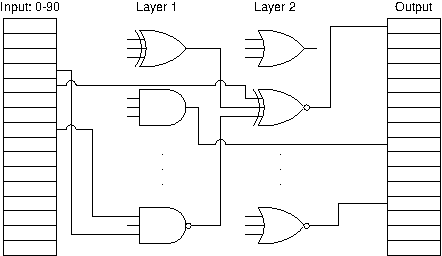
\includegraphics[scale=1.7]{cartesian_genotype}
	\caption{Genotype representation in artificial development}
	\label{fig:cartesian_genotype}
\end{figure}

The genotype of this model (fig.~\ref{fig:cartesian_genotype}) is a string of numbers that make up a feed forward circuit. This is represented as a set of four numbers where the first three points to a node, and the last number denotes which function to perform. The input to this function is the output of the nodes that the first three point to. We will see what this means in a moment.

In the simplified figure above (some gates aren't connected to avoid clutter), the input string consists of 90 bits, denoted 0 up to and including 89. Every gate, or node, are denoted 90-\emph{n}, where \emph{n} is the number of nodes. This means that the first gate we see in layer 1, is denoted 90, and the one under it is 91. Now we look at the genotype. As mentioned, it consists of four numbers. 7, 50, and 32 point to the corresponding bits in the input string, i.e.\ 7th, 50th and 32nd bits of the input string on the left. These bits are fed to the gate with a function identified by the fourth number. In this case, it is 10 - XOR. If an input number was higher than 89, it would be pointing to the output of a gate instead of the input string. The last few numbers of a genotype do not describe a circuit. They now point to either the input string or nodes. These bits make up the output string. There are no reason for why a node should be exactly four numbers. It can be any arbitrary number as long as it is consistent.

As opposed to ArtDev3D, every cellular activity is evolved. Nothing is programmed directly into the cell. Consequently, the evolved cell program can be difficult to analyze. The gates seen in figure~\ref{fig:cartesian_genotype} are just a series of Boolean operations.

\subsubsection{How it works}
There are several ways to start development with this model. One way is to represent the organism as a grid filled with cells and alternately give them maximum and no chemicals. The other way, and the way it is implemented here, is to start like ArtDev3D with a single cell and give it maximum chemicals. With the cell's and nearby cells' chemical levels, an input string is created and fed to the cell program. As the cell program is decided entirely by evolution (and chance), explanation of what happens inside the cell is nearly impossible. However, the end result is a string of numbers that determines whether or not the type of the cell should change and whether or not the cell should divide in a direction and how much chemicals the potentially new cell should be given.


\subsection{A generic development framework}
\label{sec:framework_requirements}
There are differences that can make it difficult to compare these two models. They differ not only in implementation but also in concepts and how they are represented. The most interesting thing to see here is that intercellular interactions in particular give different results in the two models.

In ADCGP, the cells communicate with each other using chemicals. The amount of chemicals exchanged, along with nearby cells' types determine what will occur in the cell in a development step. In ArtDev3D, communication happens without the chemicals. The state of the neighbourhood alone make up the external signals that contribute to determine whether or not some proteins are activated. Chemicals in ArtDev3D are used internally only and are not exchanged. Furthermore, it has shown that the number of chemical types is inversely related to fitness. Quite opposite of how ADCGP is reported to work. One can place these models on their own end of the scale. Because of this controversy, there are discussions as to whether chemicals really are necessary.

Moreover, there are other factors that come into play as well. For instance, the two models use different evolutionary algorithms, they evolve different genotypes, and the cell program is partly hard-coded in one model but not in the other. These are only two models in a relatively new field where a lot of research is still ongoing. How can we tell why something is working for one model, and not for the other? These kinds of questions can be difficult to answer with so many factors to consider.

To solve this problem, one can try and minimize the impact of these factors. This thesis proposes a framework that will provide a generic implementation of a development system that can embody any model without forcing compromises. Models that are implemented within this framework will share a common code base, making factors related to implementation and use of algorithms negligible. It will also become much clearer what one model uses or not, compared to another model.

Requirements for such a model should include:
\begin{itemize}
	\item\textbf{A genetic algorithm}

	Using a common genetic algorithm will eliminate discussions on whether or not a certain algorithm is better than another. The focus should be on the development model, and not genetic algorithms.

	\item\textbf{A development algorithm}

	Most of the models use the same basic algorithm for development, i.e.\ with every development step, every cell in an organism is told to execute their program. This occurs for a configurable number of steps, and varies very little from model to model. Hence, there is no need to implement this algorithm every time. In cases such as with ArtDev3D, this will automatically address the issue with simultaneous cell development as well.

	\item\textbf{A common messaging system}

	Especially with these two models, there are different things that go into a message that is sent to nearby cells. A common message should be able to contain most of a cell's properties while constrict the messages to just that and nothing more. The user can just choose the relevant parts for his or her model. When comparing, one should be able to say that two models differ because one uses chemicals while the other uses both chemicals and cell types.

	\item\textbf{Common concepts}

	It is important that a cell is always a cell, regardless of which model we are talking about. The definition of a cell should not change because a model wants it differently. Likewise, there should be only one definition for chemicals, organisms and proteins. While they are restricted and enforced on the user, it should also be generic enough to implement any model.

	\item\textbf{Protecting the organism}

	Access to the organism should be limited to avoid accidental tampering. Cell division will occur by telling the organism to add a cell in a particular location. This should be done through a function call. All information regarding the cellular neighbourhood should be available through the messaging system. As such, mechanisms should also be available to check whether a cell in a particular location exists or if it will be occupied by a new cell. This is to enable checks prior to performing cell division.
\end{itemize}

There are several benefits to using such a framework. First and foremost, it will cut down on implementation time. Such a model will allow a user to concentrate wholly on their model and not spend time implementing the most suitable genetic algorithm, or finding out whether or not the messaging system was implemented correctly. Instead, the user need only use what is already there and just fill in the blanks. Secondly, the implementation can be guaranteed to work. As the framework matures, the user can be assured that if something does not work, it is most likely their model and not because of a bug elsewhere in the system. Finally, and probably most importantly, the framework will hopefully be able to reduce the number of factors that prevent a clear verdict on a comparison.

We've seen that these two models are quite different from one another, which is why they will serve as an excellent starting point to implement the framework. One of the criteria for the framework is to be generic as it should be able to implement any model conceivable. It should also be able to perform at least as well as the original implementation did. We shall have a closer look at this in the next chapter.

	\section{Implementation}
\label{sec:implementation}
In this chapter, we will introduce the genetic engine that will lie the basis for the development framework. Much of the focus will lie on performance and making things logical. A brief introduction to using the framework will be held. We will also have a closer look at the two models discussed in the previous chapter. This time around, it will be a little more technical.


\subsection{About Ngene}
\emph{Ngene} is a flexible, generic, multi-purpose genetic algorithm engine written in C++ with heavy emphasis on performance and flexibility. The engine is divided into logical modules that can easily be interchanged or extended upon in order to fit the intended purpose. A sub-goal of this engine is also portability. Anybody should be able to use this engine on their platform of choice, regardless of whether they are sitting on Microsoft\textregistered Windows\texttrademark or Unix, and hardware based on Intel\textregistered Architecture or Power Architecture.

The prototype for this engine started out as an assignment for a sub-symbolic artificial intelligence course. It was written in Python, which later proved to be too slow for this kind of application, and later partially ported to C++ because I wanted to learn the language at the time. The project got lost in a pile of other assignments and was never heard from again. The engine was finally picked up again, re-designed and completed for the purpose of this thesis.

\subsubsection{Modular Design}
The modular design of Ngene is the heart of it all. In order to achieve maximum flexibility, the engine should be able to change any of its parts without having to do anything special. Should the user feel like changing the mutation method, this should be as easy as changing a single line in a configuration file. This is most useful because different experiments may require different genotypes or any other modules. With that in mind, the design is therefore broken into the following logical modules:

\begin{itemize}
	\itemsep=0pt
	\item\textbf{Core} - The genetic algorithm itself
	\item\textbf{Fitness} - Assesses the fitness of a genotype
	\item\textbf{Genotype} - Generates the genotype and translates them to phenotype
	\item\textbf{Mating} - Crosses two genotypes
	\item\textbf{Mutator} - Mutates a genotype
	\item\textbf{Selector} - Randomly selects a genotype
\end{itemize}

Each of these modules are like the parts of a car. Roulette selection can be exchanged for tournament selection, just like how the motor can be exchanged for another to enhance its performance. Of course, without the technical difficulties involved when changing a car engine. This modular design will allow users to swap a module without prior knowledge of programming. In fact, writing code will not be needed at all unless a new module is required. This design will also keep the code much cleaner and easier to maintain.

\subsubsection{Why C++?}
In a sense, one can say that this project was made possible because of my prototype in Python. It taught me many higher level concepts that is practically non-existent in lower level languages such as C++. Without it, I probably wouldn't have been able to bring the project to the level it is today. Especially without the concept of a dynamic type, the idea of a container that can contain anything from an integer, to a string, to a floating type number, I would still have trouble trying to compensate for it with complex algorithms to deal with raw data pointers. Most importantly, it taught me the importance of optimization and use of libraries.

Choosing a programming language depends on what kind of application you want to write. A simple program with no special requirements can be written in any language. For instance, a mail client written in Python will perform equally well as any other client because the focus lies on fetching and displaying e-mails and the ability to manage them in an easy way. The features are more important than the extra two milliseconds it takes to perform a query. However, there are applications for which performance is more important than anything. Arguably, such programs should be written in one of two ways: In assembly (or machine code) or C/C+. While assembly is rarely used these days due to being practically unreadable for mortals, C and C++ is often used for time critical applications. Unlike languages that depend on a virtual machine (C\#, Java), or an interpreter (some LISP dialects, Python), code written in C/C++ is compiled directly to machine code before executed, often yielding much better performance.

C++ is thought of as being a middle level language. It has the advantages of both the lower (machine code) and higher level languages, but also the inherent disadvantages. For example, all memory management must be explicitly handled in the code. C++ does not have a garbage collector typically found in higher level languages. This means that we have to be extra careful of de-allocating memory to avoid leaks, and prevent access of invalid memory addresses. Furthermore, C++ doesn't come with as big a convenience library as those found in aforementioned languages. Such libraries save a lot of time, eliminating rewriting often used algorithms and the headache of debugging faulty code. Fortunately, efforts are being made to ease the implementation through external libraries.

\subsubsection{Boost C++ Libraries}
\emph{Boost}\footnote{\url{http://www.boost.org/}} is a collection of libraries which complement the C++ Standard Library (STL). Ngene makes use of this collection, saving time and effort, and guaranteeing that such code works as it should.

\paragraph{\textbf{Boost.Any}}\cite{henney2001}
A problem with writing a generic genetic algorithm in a strongly typed programming language, is that different studies require different data types to be passed around the system. CGP, for instance, uses integers to implement its genotype, while ArtDev3D uses a custom defined type. In other models, there may even be a mix of different types. It is impossible to foresee what may or may not be used, and we are thus forced to abstract this away. Unfortunately, C++ will not allow an integer variable to store any other data type than an integer. In a higher level language like Python, there exists a container that can store any type of data:

\begin{verbatim}
>>> foo = 1 + 2
>>> print foo
3
>>> foo = "awesome"
>>> print foo
awesome
>>> _
\end{verbatim}

Doing something similar in C++ would simply give us a syntax error. To make such a container in C++, will require some coding. Fortunately, this has already been implemented and is freely available as part of \emph{Boost}. The modular design would otherwise not work without it, at least not within given time constraint. The container, called \emph{Boost.Any}, does not differ much from the one found in Python and comes only at the cheap cost of requiring a type-casting before the data can be handled as normal.

\paragraph{\textbf{Boost Random Number Library}}\cite{maurer2000}
Another problem with genetic algorithms and development in general is implementing a good pseudo-random number generator. Ngene uses the implementation of \emph{Mersenne twister} pseudo-random number generator also found in the Boost libraries. This generator was chosen for its long period ($2^{19937}-1$ or approximately $4.3*10^{6001}$), and because it is relatively fast compared to other algorithms. It also passes a number of tests for randomness, including Diehard\footnote{A collection of tests to measure the quality of the randomness of the generator, developed by George Marsaglia.} and most of the stricter TestU01 Crush\footnote{Another collection of tests, developed by Pierre L'Ecuyer and Richard Simard.} randomness tests.

\subsubsection{Brief System Overview}
\begin{figure}[!ht]
	\centering
	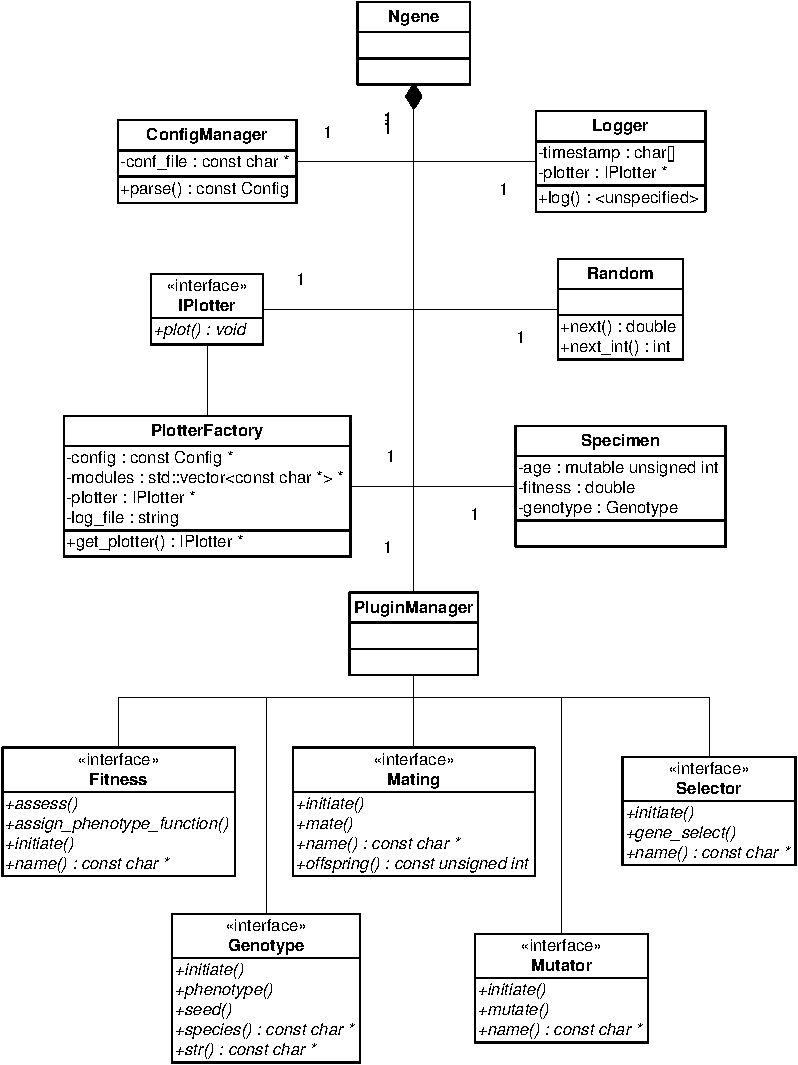
\includegraphics[scale=0.9]{diagram_ngene}
	\caption{Overview of Ngene}
	\label{fig:diagram_ngene}
\end{figure}

Figure~\ref{fig:diagram_ngene} shows a brief overview of how Ngene is put together. At start-up, three of these parts are responsible for what must take place before anything can be run in accordance with the user's parameters. \texttt{ConfigManager} takes care of reading the configuration file and creating a settings object that every other parts have access to. Once the configuration file has been parsed, \texttt{PluginManager} will use this object to find out which modules it's going load. If the user specified tournament selector, it will load the tournament module and make it ready for the genetic engine. When every module is loaded, \texttt{Logger} will use the same settings object to find out how it should log the current run, whether it should plot a fitness/generation graph or just print out the progress on the screen. By now, the genetic algorithm will start. It is a very simple algorithm:

\begin{enumerate}
	\itemsep=0pt
	\item An initial population is randomly generated.
	\item \texttt{Specimen}s are randomly selected for crossover.
	\item A configurable percent of the offspring are mutated.
	\item Repeat step 2 until the offspring population is of satisfactory size.
	\item Replace adult population with offspring population.
	\item Repeat process from step 2 until the maximum number of generations is reached, or a perfect \texttt{Specimen} is found.
	\item Write log/graph and final \texttt{Specimen} to disk.
\end{enumerate}

The final step is the responsibility of \texttt{Logger}. \texttt{Logger} has no knowledge of what format the \texttt{Specimen} should be written as. Be it a text file, an image or a proprietary format, it will simply request the \texttt{Genotype} module to give it some data to write to disk. The output format is actually coded in each \texttt{Genotype} module because it rarely changes for a single experiment and/or model. Otherwise, a new module must be written anyway.

\texttt{PluginManager}, along with the responsibilities of loading and releasing modules, will also act as a layer between the modules and the genetic engine itself. The engine will never have to bother with the specifics of each module. It should be able to just tell what a module ought to do. Of course, this requires that the modules implement a predefined interface in order to be compatible with this layer. These are described in more detail in the appendix.


\subsection{Ngene Development Framework}
\begin{figure}[!ht]
	\centering
	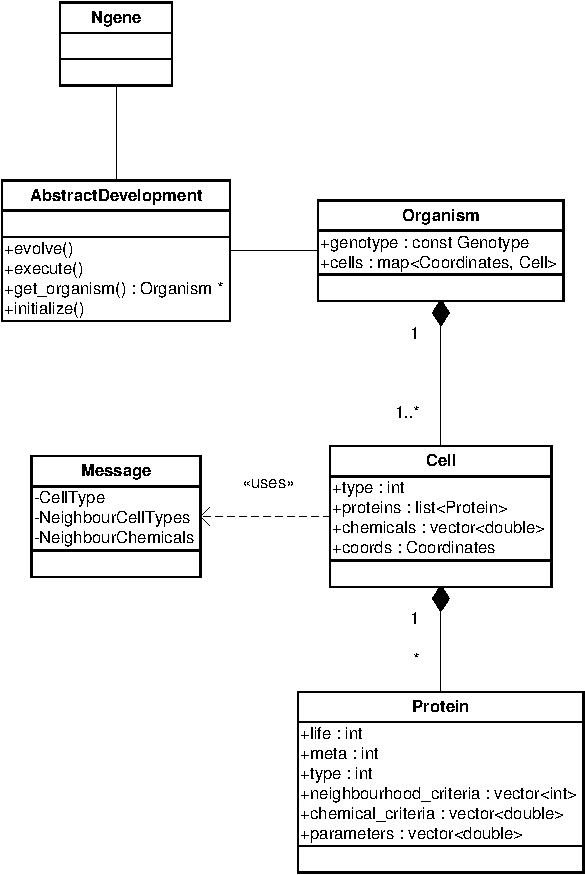
\includegraphics{diagram_ndevframe}
	\caption{Overview of Ngene Development Framework}
	\label{fig:diagram_ndevframe}
\end{figure}

The downside of having such a flexible design, is that users are given too much freedom in implementing their own modules, making it difficult to compare two models without having to factor in differences in implementations. A common generic development framework can remove these factors and ease the implementation at the same time. The Ngene Development Framework is an attempt of such a framework.

The framework provides a code base that implements a common development algorithms, along with common concepts such as a cell and protein. Figure~\ref{fig:diagram_ndevframe} shows how they are defined. We see that a cell is defined to have a type, proteins, chemicals and messages. These properties may be fixed but users can choose to not use them. ADCGP, for instance, does not make use of proteins. \texttt{AbstractDevelopment} is the class that implements development algorithm. As mentioned in chapter~\ref{sec:framework_requirements}, it implements functions that protects the organism: \texttt{divide\_cell()}, \texttt{exists()}, \texttt{queued()}. They add a new cell, checks if a cell exists in given location and checks if there will be a new cell in given location, respectively. Most of these functions are already implemented and ready to use. Only \texttt{initialize()} and \texttt{execute()} are not. Their function is described in more detail in the following subsection.

An intercellular communication algorithm is also included. This works by providing a number of information that can be exchanged. In figure~\ref{fig:diagram_ndevframe_msg}, we see that a message can consist of cell type and chemicals. Some models, say model A may only use the chemicals part of the message while discarding everything else. For model B or C, this might not be the case. As we saw earlier with ArtDev3D and CGP, the communication between the two differs a lot. It is important that the message system can provide what is needed for any system and still be able to clearly distinguish the differences so that we can easily take this into consideration when comparing the two models. Use of this code base is enforced in order to ensure that all comparison made between different development models are based on a common ground.

\begin{figure}[!ht]
	\centering
	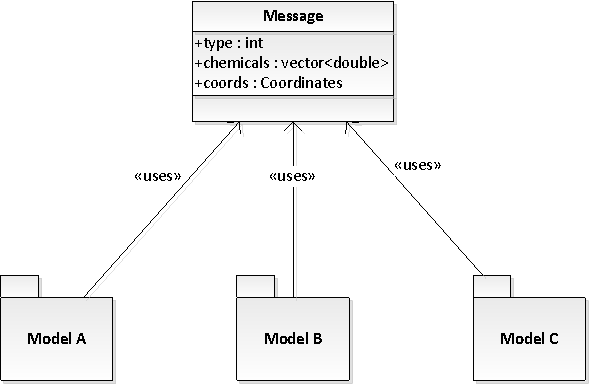
\includegraphics{diagram_ndevframe_msg}
	\caption{A common message implementation should let users easier distinguish the differences in intercellular communication between different models.}
	\label{fig:diagram_ndevframe_msg}
\end{figure}

Figure~\ref{fig:diagram_ndevframe_common-base} demonstrates this requirement. We can see right away that all three models differ because model A and B use chemicals, while C uses proteins. We also see that model B and C require a control program in addition to their cell programs. When models are implemented using the framework, we will be able to clearly see which parts a model uses and why it is unique compared to another model. Since a common code base is used, you can, for example, no longer say that these models produced different results because they ran through different development algorithms.

\begin{figure}[!ht]
	\centering
	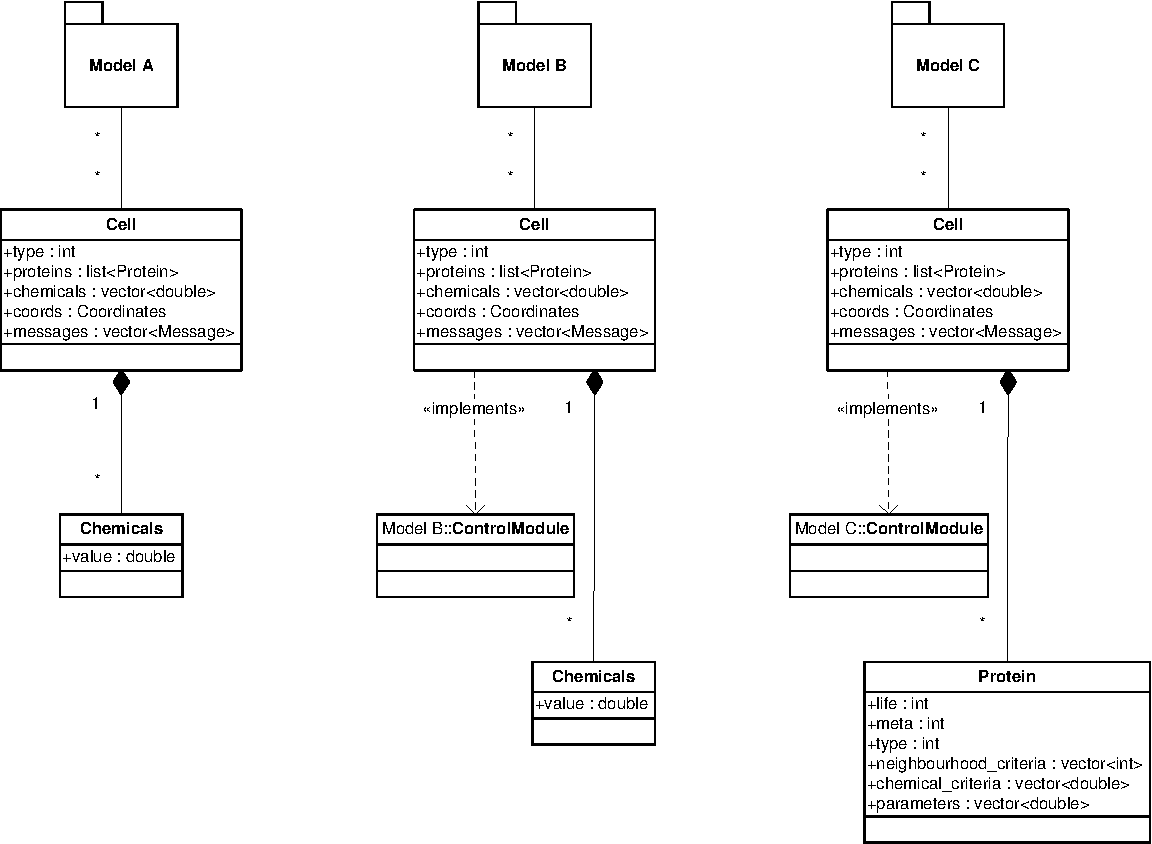
\includegraphics[scale=0.9]{diagram_ndevframe_common-base}
	\caption{Albeit different, all three models still use the same implementation of a cell, chemicals and proteins, and receive the same messages.}
	\label{fig:diagram_ndevframe_common-base}
\end{figure}

Since the framework is going to be used by many users, speed is also a concern when designing it. It is important that the framework is not only flexible and easy to use, but also perform relatively well compared to other implementations. Lots of thought as been put into how to represent the organisms themselves. In the current implementation, a C++ Standard Library (STL) \texttt{<map>} is used to store the cells using their coordinates as the key value. Other alternatives were also considered:

\begin{center}
	\begin{tabular}{ r | c | c | c }
		~ & STL \texttt{<map>} & STL \texttt{<vector>} & STL \texttt{<ext/hash\_map>} \\
		\hline
		element access & $O(log~n)$ & $O(1)$ & $O(1)$ \\
		\hline
		insertion & $O(log~n)$ & $O(1)$ & $O(1)$ \\
		\hline
		search & $O(log~n)$ & $O(n)$ & $O(1)$ \\
	\end{tabular}
	\label{tbl:speed}
\end{center}

A quick glance at the comparison table and the \texttt{<ext/hash\_map>} may seem like the best choice to go with. However, there are some drawbacks that must be taken into consideration.

A hash table creates a unique key based on a number of properties found in the value to be stored. The key is used to retrieve the value at some later point. The hashing algorithm is essential in both that it determines how uniform the distribution will be over the array, and how well the hash table will perform overall. A too simple hashing algorithm will often experience collisions, i.e.\ a lot of values will have the same key. When this occurs, there are several ways to handle it (also called collision resolution). In worst case scenario, the key will point to a list, thus making the hash table perform like a linked list. Insertion is still constant but lookup may be as bad as $O(n)$. On the other hand, an overly complex hashing algorithm will also deteriorate performance because more CPU cycles is spent calculating a good hash value. Regardless of how good the hashing algorithm is, collisions will always occur. The \emph{birthday paradox} predicts that it doesn't take many elements before the chance of a collision exceeds 95\%, even for very big arrays. It is clear that the hash table cannot guarantee its performance advantage over the other containers. Besides, for the experiments conducted in this thesis, the number of cells rarely exceeded 1000. If we use a \texttt{<map>}, which is the case here, it will take at most ten comparisons to find an element by its key value. A good hashing algorithm will use approximately the same number of operations to calculate a key value, perform lookup, and resolve any collisions.

The problem with \texttt{<vector>} is that it is one-dimensional. This makes it difficult to efficiently calculate x, y and z values of a coordinate since we don't know how many cells there will be. Another drawback is that it will take $O(n)$ time to look for neighbours. This can be worked around by maintaining an up to date neighbours list for every cell. This will make lookup $O(1)$ but increase insertion time to $O(n)$. \texttt{<map>} offers easier facilities to perform such tasks more efficiently. Later, in chapter \ref{sec:improvements}, we will discuss a custom implementation that will theoretically perform better than mentioned containers.


\subsubsection{Using the Framework}
\begin{figure}[!ht]
	\centering
	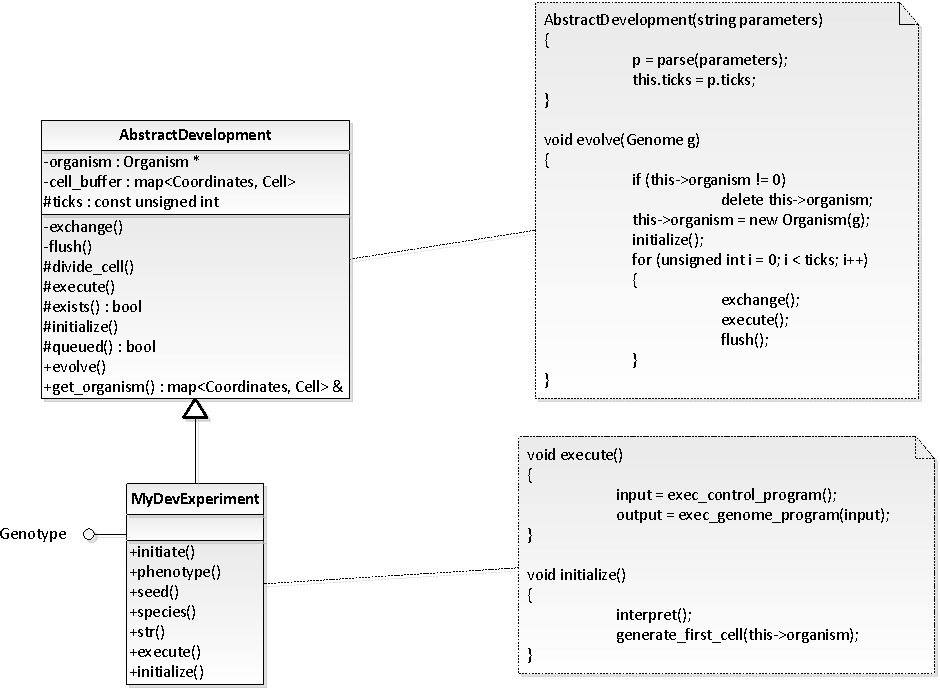
\includegraphics{diagram_ndevframe_ex}
	\caption{An example of how one can implement \texttt{MyDevExperiment}.}
	\label{fig:diagram_ndevframe_ex}
\end{figure}

The framework was designed to ease the implementation effort as much as possible. The whole code base can be inherited from \texttt{AbstractDevelopment}. To port a model to this framework, only two functions need to be implemented: \texttt{execute()} and \texttt{initialize()}. The latter is executed once with every new organism that is to be developed, and can be used to unpack the genotype to a cellular program and/or generate initial cells in the organism. \texttt{execute()} is called every development step/tick, for every cell in the organism. Here, the cell program from the genotype can be executed as well as any control programs that might be needed. Note that any messages sent has already been received and are stored in the cells by the time any cell is given the chance to fulfill its purpose in a tick. It will not be possible to actually access the organism itself from this function. This is to avoid accidental tampering of the organism. There is an example implementation of these two functions in figure~\ref{fig:diagram_ndevframe_ex}.

For the purpose of this thesis, two models were implemented within this framework not only to test the flexibility and performance of this framework but also to see what is missing and what areas need improvement. It is therefore important that these models represent the widest spectrum of computational development.


\subsubsection{ArtDev3D}
\label{sec:Implementation:ArtDev3D}
Porting Johan H{\o}ye's master's thesis\cite{hoye2006} to Ngene's framework has been a matter of finding out what occurs in a cell during a development step, and whether or not there are external processes that needs to be accounted for. As described in chapter~\ref{sec:Models:ArtDev3D}, the genotype of the model does not do all the work in a cell. The cell has its own control program as well. The program can be summarized as the following steps:

\begin{enumerate}
	\itemsep=0pt
	\item Clear all queued actions.
	\item For every active protein, queue their action requests.
	\item Accumulate actions (add them together to execute in one go).
	\item Execute action \#1: Transcribe proteins.
	\item Execute action \#2: Regulate chemical levels.
	\item Execute action \#3: Perform cell division.
	\item Execute action \#4: Change cell type.
	\item Remove dead proteins.
\end{enumerate}

The implementation of the model might seem overwhelming at first impression. There is a heavy use of biological concepts in the code and the simplest operation may span across many classes, and files, as a result. This alone makes it hard to follow the code flow, but the little system documentation that does exist, fortunately, does provide some help though it consists mainly of commentaries in the source files themselves. While his efforts in making it understandable are visible, it might be beneficial to flatten the structure a bit and get rid of some of the redundant structures that are inspired by nature. There is another reason for why this was altered as well.

In theory, such an implementation can have a negative impact on performance. When a simple operation performed must call a function to call another function to call yet another function and so on, can put the calling stack under strain. This may occur because this does not happen only once, but several times every development step in a single cell. And as we know, there are plenty of cells in an organism. Flattening the structure as mentioned, will reduce the number of calls and potentially improve performance.

\begin{figure}[!ht]
	\centering
	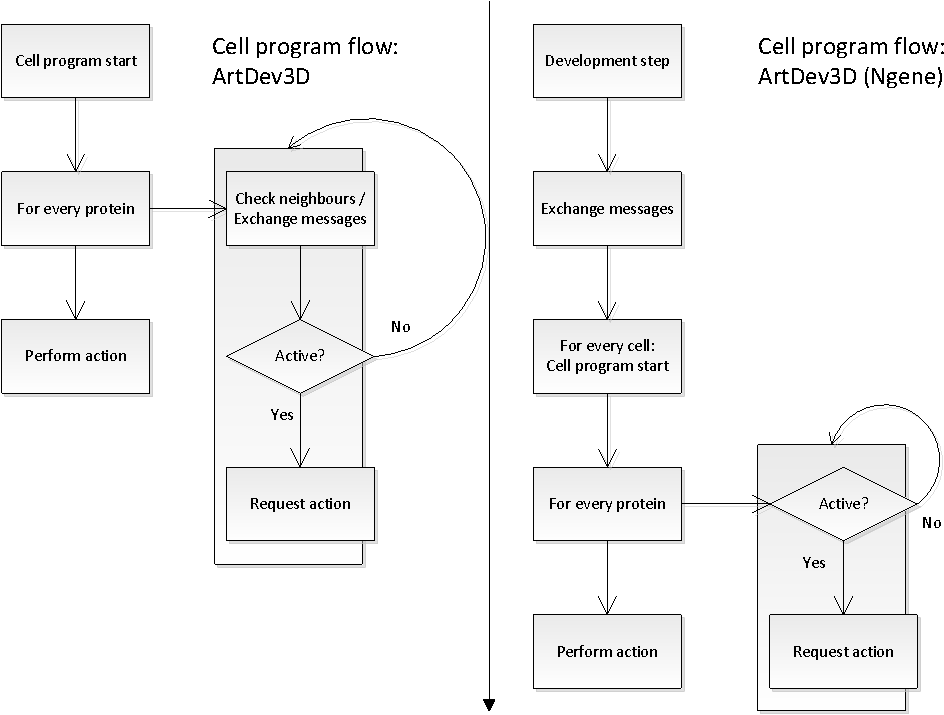
\includegraphics[scale=0.9]{artdev3d_flow}
	\caption{On the left, original ArtDev3D flow. The changed flow on the right.}
	\label{fig:artdev3d_flow}
\end{figure}

There was also an issue that was identified and patched in the port. In most models, cells are developed simultaneously. In order to achieve this, information must be exchanged between all cells before a cell can execute its functions. This is to ensure that the cell program will execute based on the current state of the organism without interfering for other cells. In ArtDev3D, this is not properly implemented. The left logical flow in figure~\ref{fig:artdev3d_flow} shows the original ArtDev3D implementation. Upon execution, the cell will start collecting requests from its proteins. The proteins can request an action when they are activated, i.e.\ when the state of the cell and its neighbours are above a threshold. The requests are queued up and then executed. The problem with this, is that it all happens in a single step. Thus, cells that already have had their turn before the current cell, will have an altered state. Actions are therefore based on a mix of ``newer'' information from these cells, and ``old'' information from the rest. When porting this code to the new framework, the cell will no longer have direct access to other cells. Instead, it will receive messages from (or a snapshot of) nearby cells before the development step takes place in any cell. The right logical flow in figure~\ref{fig:artdev3d_flow} is the altered flow of ArtDev3D. Messages are exchanged before any cells are given control. Any action requests are then based on information that does not change as previously. This change may alter the outcome of the model but was addressed because the development algorithm of the framework is already implemented. The model is merely a user of it now.


\subsubsection{Artificial Development (ADCGP)}
\label{sec:cartesian}
This model was implemented from scratch with help from Dr. Julian F. Miller. The model is rather simple because the whole cell program is in the genotype. The implementation should only need to translate the genotype into a working digital circuit and be able to use it.

The genotype is an array of integers. The number of integers depend on the number of layers and how many nodes each layer consists of. The number of layers and nodes per layer is static. This will keep it simple, and also make the crossover less complicated. As far as I know, this should be in line with Dr. Miller's implementation as well. Each node consists of four integers - three that will serve as connection points to other nodes while the last one will point to a specific function. The function will get its input from the connected nodes' output. The functions implemented here are basic Boolean operations, in addition to the four elementary mathematical operations.

\begin{itemize}
	\itemsep=0pt
	\item \texttt{AND}, \texttt{MUX}, \texttt{NAND}, \texttt{NOR}, \texttt{OR}, \texttt{XNOR}, \texttt{XOR}
	\item addition, division, multiplication, subtraction
\end{itemize}

Upon initialization, the engine will receive the genotype and will start translating it into a digital circuit. The cell program is then executed:

\begin{itemize}
	\itemsep=0pt
	\item An input bit-string is generated from the chemical levels and types of the current cell together with its neighbours.
	\item The bit-string is sent to the cell program.
	\item The output bit-string is parsed. Some bits will give the cell a new type, the rest will tell the cell to divide in particular directions and how much chemicals these will receive.
	\item The number of chemicals in the cell is adjusted using this formula

	$(c_{ij})_{new} = \frac{1}{2}(c_{ij})_{old} + \frac{1}{16}\sum_{k, l \in N} (c_{kl})_{old}$,

	where $(c_{ij})_{old}$ is the current chemical level, $(c_{ij})_{new}$ is the new chemical level and $\sum_{k, l \in N} (c_{kl})_{old}$ is the sum of the chemical levels in nearby cells (defined as the eight immediate neighbours in 2D grid space).
\end{itemize}

The input bit-string consists of 90 bits. The first 72 bits are the chemical levels in the cell and its eight immediate neighbours (8 bits each). The last 18 bits are the types of the cell and its eight immediate neighbours (2 bits each).

The output bit-string consists of 74 bits. 2 bits denotes the type that the cell changes into. The following 8 bits tells which directions the cell will duplicate itself to (1 bit for each direction). How much chemicals these cells will have are determined by the last 64 bits (8 bits for each direction).

Dr. Miller has also provided with important information regarding his implementation of the model. His implementation actually contains a bug that causes the program to only read the most significant bit from the chemical bits in the neighbours. The other bits are set to zero. When he later identified and patched this bug, he found that the bug was actually beneficial to the model. This bug was also re-implemented in order to make it closer to the original implementation.

	\section{Experiments}
\label{sec:experiments}
Porting the models to the new framework is only the first part of the project. It is also important that these models, once ported, are able to perform in the exact same way as the original code would. The best way to verify that it does, is to repeat a small sample of experiments and compare the results to the original reports. A smaller test was also conducted to measure the performance of this framework. This test will show whether the improvements to ArtDev3D proposed in the previous chapter actually does make it faster.

TODO:
you need to present the experiments in a slightly different light. Your goal is to test the platform to make sure that is works towards its goals. You re repeating but not exactly - you are not just rerunnign their experiments on their platform as the header would imply. 4.1. Developing 3D shapes using ArtDevsD model...etc. In intro yu can describe the fact that the gals is to replicate the experiments n a differnet platform to illustrate the viability of the platform for that model. Similar with the Julian model.


\subsection{Developing 3D shapes using ArtDev3D's model}
For this model, the sphere and the x-mas tree was chosen to test the new implementation of ArtDev3D. The reason for this is because the sphere is a relatively simple shape to evolve and easily achieve perfect fitness. The reason the normal tree is not chosen is because they are almost the same in complexity and ArtDev3D equally well on both of these. For the second test, we want see how well the new implementation will do on difficult shapes.

Both of these experiments were conducted with different settings in order to see how parameters would affect the fitness of the individuals. In this thesis, however, I used a fixed set of parameters for simplicity's sake. The numbers may therefore deviate from the original results. Both of these experiments are run with settings as close to the original experiments as possible:

\begin{itemize}
	\itemsep=-2pt
	\item Population: 1 000
	\item Generations: 500
	\item Mating rate: 90\%
	\item Mutation rate: 10\%
	\item Crossover: Single point
	\item Selection: Tournament (size=4, pressure=0.8)
\end{itemize}

And the parameters used for development:

\begin{itemize}
	\itemsep=-2pt
	\item Development time: 12 ticks
	\item Protein lifespan: 5 ticks
	\item Cell types: 1 (sphere) / 12 (x-mas tree)
	\item Chemical types: 1
	\item Don't-care-neighbours: 6
\end{itemize}

Both of these experiments were run 200 times. H{\o}ye reported to have run these experiments 980 times each but with varying parameters. Considering there are several set-ups he could have run them with, a smaller number was chosen now because only one set-up is used. 200 runs should be enough to demonstrate the point of this chapter.

\subsubsection{Sphere}
\begin{center}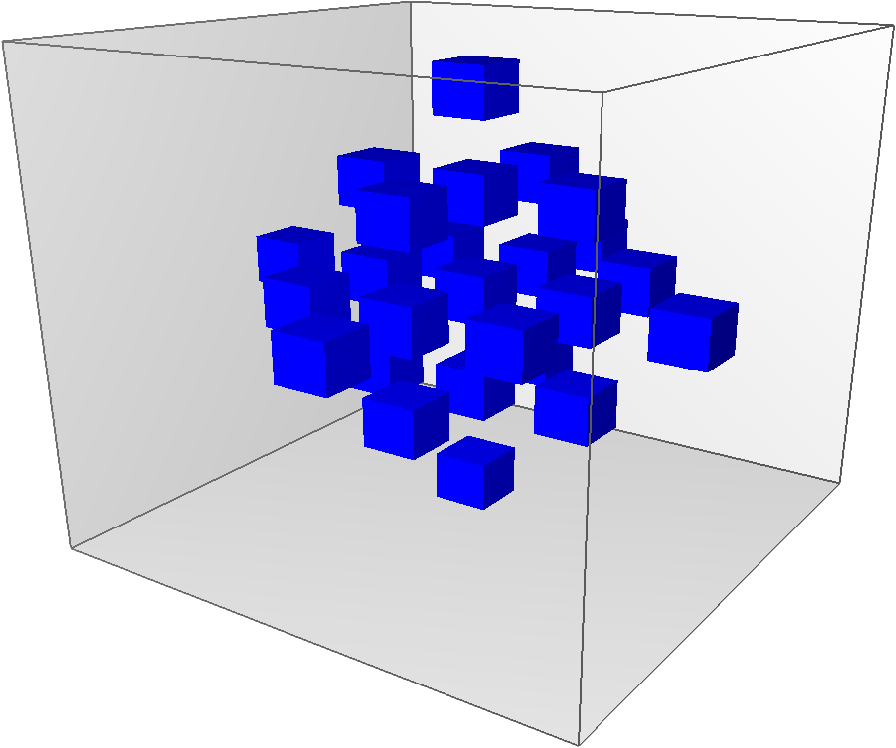
\includegraphics[scale=0.2]{sphere}\end{center}
This shape seems the simplest to evolve as it is entirely symmetrical and much less complex than other shapes. Since these experiments are about verifying that everything runs as it should, they will always use the same parameters. The number of perfect specimens found was recorded and presented in figure~\ref{fig:chart_artdev3d_sphere}.

\begin{figure}[!ht]
	\centering
	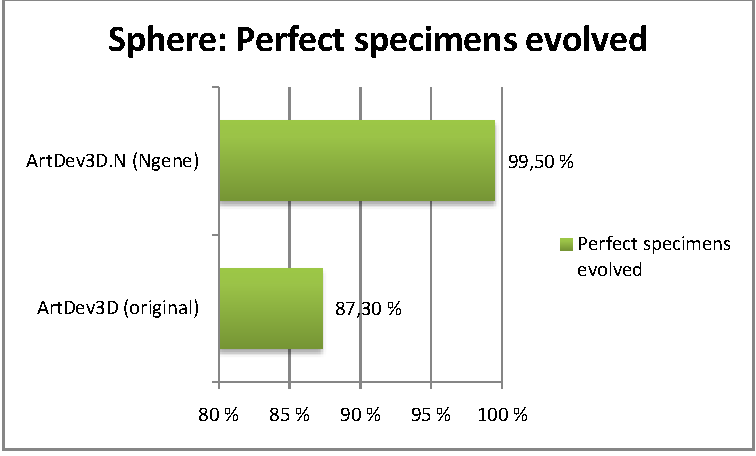
\includegraphics[scale=0.9]{chart_artdev3d_sphere}
	\caption{ArtDev3D: Sphere results}
	\label{fig:chart_artdev3d_sphere}
\end{figure}

Original ArtDev3D managed to evolve perfect fitness 856 out of 980 experiments. It is important to remember that these were run with \emph{different} settings whereas we are using the best settings available here. That is why we see a much higher percentage (199 out of 200) than the original experiments. Had we known what these parameters were beforehand and used them, the number would probably have been much closer to the original results. Regardless, it does show that Ngene can perform equally well.

\subsubsection{X-mas tree}
\begin{center}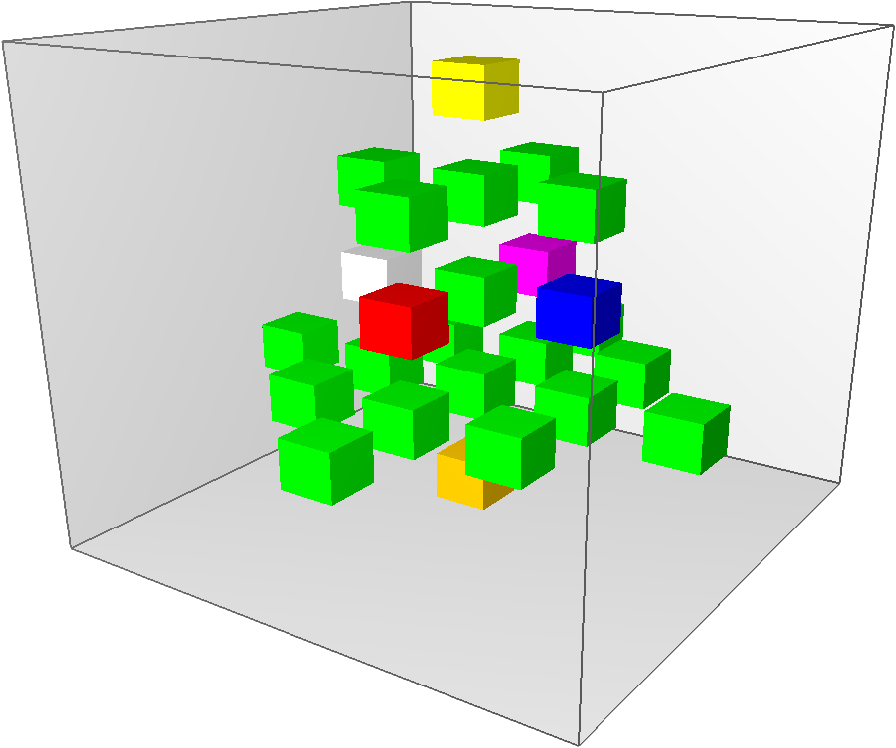
\includegraphics[scale=0.2]{x-mas-tree}\end{center}
This experiment is of a different nature than the previous one. It may not be very scientific but should demonstrate how well Ngene performs on complex shapes compared to ArtDev3D. No perfect specimens are expected here because ArtDev3D had a hard time evolving one, and it is not expected for Ngene to outperform it. The highest fitness after each run was recorded for figure~\label{fig:chart_artdev3d_x-mas-tree}.

\begin{figure}[!ht]
	\centering
	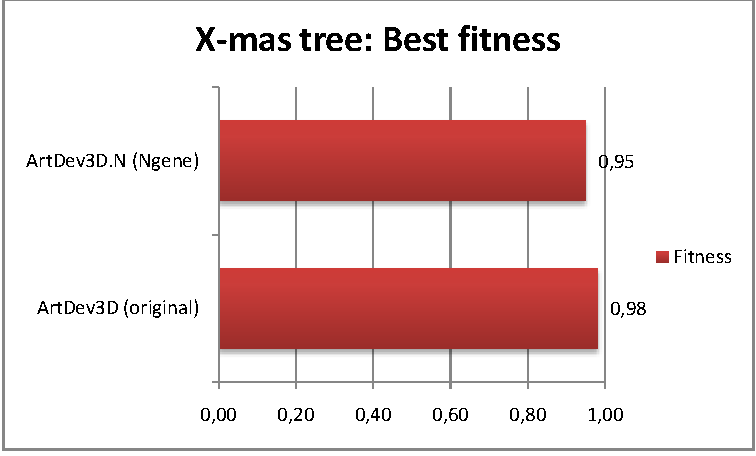
\includegraphics[scale=0.9]{chart_artdev3d_x-mas-tree}
	\caption{ArtDev3D: X-mas tree results}
	\label{fig:chart_artdev3d_x-mas-tree}
\end{figure}

It seems that Ngene is performing rather well. Note that the highest fitness achieved in ArtDev3D only occurred once in the 980 test runs conducted. This experiment is but a fifth of that, and it is not inconceivable that Ngene might be able to achieve higher fitness with a larger sample. Interestingly, Ngene only managed to evolve fitness above 0.9 in 57 out of 200 runs. The rest were above 0.8 however.

\subsubsection{Summary}
We've seen that Ngene's implementation of ArtDev3D can evolve on an equal level as the original implementation. In chapter~\ref{sec:Implementation:ArtDev3D}, I've mentioned that there was a fix applied to the engine when it was ported to the framework. From what can be seen above, it would seem that this patch has not affected the model in any perceivable way. Whether or not the fix is beneficial in any way, is difficult to see. It may very well be that the bug is dormant.


\subsection{Developing the French flag using artificial development}
For the ADCGP model, the French flag experiment was picked out. The purpose of this experiment is to evolve a grid of cells that resembles the French flag. Each cell is given a type of either blue, red or white. For every cell that corresponded with the target, one point was rewarded. The fitness is calculated from the total points scored divided by maximum score achievable. The engine ran with the following settings:

\begin{itemize}
	\itemsep=-2pt
	\item Population: 100
	\item Generations: 10 000
	\item Mating rate: 90\%
	\item Mutation rate: 30\%
	\item Crossover: Single point
	\item Selection: Tournament (size=4, pressure=0.8)
\end{itemize}

The target phenotype used:

\begin{center}\fbox{
\includegraphics{French-flag}}\end{center}

Finding the right development time for this particular problem proved to be rather difficult. It would seem that setting the development time too high not only slowed down the whole process, it also made it harder for the organisms to evolve correctly. The experiments started out with development time of 10 ticks and was slowly decremented as the results were not satisfactory. The following are the best evolved organisms using 4 ticks.

\begin{center}
	\fbox{
\includegraphics{cartesian-4-3-90-9-3-20081119-083309}}
	~\fbox{
\includegraphics{cartesian-4-3-90-9-3-20081119-091139}}
	~\fbox{
\includegraphics{cartesian-4-3-90-9-3-20081119-230852}}
\end{center}

It seemed odd that setting the development time one step longer would have any saying in how the organisms would grow. To ensure that the results weren't purely coincidental, the experiment was repeated once more for five ticks.

\begin{center}
	\fbox{
\includegraphics{cartesian-5-3-90-9-3-20081120-221123}}
	~\fbox{
\includegraphics{cartesian-5-3-90-9-3-20081120-233001}}
	~\fbox{
\includegraphics{cartesian-5-3-90-9-3-20081121-002613}}
\end{center}

These results seem to suggest that the model is not stable. Colours appear in areas they shouldn't be in as opposed to the previous results where the colours at least stayed closer to each other. One can theorize that the growth continues even after target phenotype have been evolved, hence resulting in a worse fitness. This seems to be backed up by the fact that the engine would more frequently obtain fitness above 0.9 when using development time of four when compared to five. Using development time of 10 also raised the number of cells above 200.

To further investigate this issue, the phenotype was altered so that it would have a border around the flag.

\begin{center}\fbox{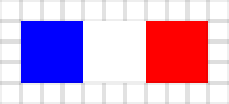
\includegraphics{French-flag-border}}\end{center}

This new phenotype will hopefully show whether or not the model does continue to grow, or if it manages to maintain a status quo to some extent. No changes were made to the settings above. The tests were repeated using the new target phenotype.

\begin{center}
	Development time: 4 ticks\newline
	\fbox{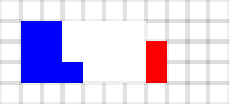
\includegraphics{cartesian-4-3-90-9-3-20081120-071044}}
	~\fbox{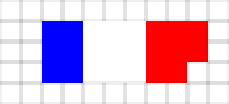
\includegraphics{cartesian-4-3-90-9-3-20081120-081439}}
\end{center}

\begin{center}
	Development time: 5 ticks\newline
	\fbox{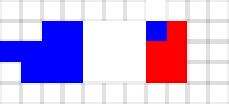
\includegraphics{cartesian-5-3-90-9-3-20081121-063215}}
	~\fbox{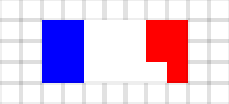
\includegraphics{cartesian-5-3-90-9-3-20081121-072947}}
	~\fbox{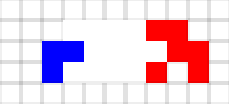
\includegraphics{cartesian-5-3-90-9-3-20081121-205507}}
\end{center}

As suspected, the average fitness dropped due to the increased size and complexity of the phenotype. With the exception of the first flag in the second row that ``bleeds'' into the border (two cells: blue on the left and white cell above the one blue cell in red cells zone), all of them are missing cells for some reason. It seems like the model compensates by either growing less cells or initiating cell death more often. Unfortunately, the results can't be called conclusive due to the nature of test. One will have to look into how the organisms change in each development step. The tools necessary for this is unavailable at the moment.

Another interesting thing to note is that the bug mentioned in section~\ref{sec:cartesian} had little to no effect on any of the results above. In fact, the no-bug version seem to achieve higher fitness more frequently than the bugged version by a small margin. This conflicts with what Dr. Miller reported.


\subsection{Performance Benchmarks}
With regards to what has been written about ArtDev3D up to this point, I've only discussed the potential performance gain of this framework without showing anything concrete. We shall now put these claims under scrutiny, and see how fast the new ArtDev3D, cleverly dubbed ArtDev3D\emph{.N} (N for Ngene or N-hanced), really is. This simple benchmark test was run on an Intel\textregistered Core\texttrademark 2 Duo E6300 with 2 GB of DDR2-RAM under Linux 2.6.27-7. The conditions of the programs under run:

\begin{itemize}
	\itemsep=0pt
	\item ArtDev3D ran with Java\texttrademark SE Runtime Environment 6 Update 10 build 33.
	\item ArtDev3D.N was compiled with GCC 4.3.2, with optimization flags: \texttt{-O3}.
	\item Additionally, ArtDev3D.N was also compiled with Intel\textregistered C++ Compiler (ICC) 11.0 build 069, with optimization flags: \texttt{-xHost -fast}.
\end{itemize}

The same settings were used for both engines:

\begin{itemize}
	\itemsep=-2pt
	\item Population: 100
	\item Generations: 100
	\item Mating rate: 90\%
	\item Mutation rate: 30\%
	\item Development time: 12 ticks
	\item Target: Sphere
\end{itemize}

Perfect termination was disabled so that the engines would not exit when perfect fitness was found. This is to ensure that both engines ran for the exact same number of generations. The test was repeated 100 times and the average time was then calculated.

\begin{figure}[!ht]
	\centering
	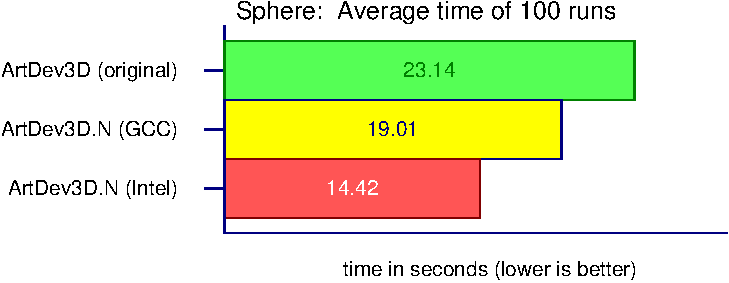
\includegraphics[scale=0.9]{chart_avg-time}
	\caption{ArtDev3D vs. ArtDev3D.N: Speed}
	\label{fig:chart_avg-time}
\end{figure}

The speed gained (fig.~\ref{fig:chart_avg-time}) here is quite significant considering that the sample is relatively small to perform a benchmark on. Using an open source compiler such as GCC, Ngene is faster than ArtDev3D by 4.13 seconds. This is to be expected as C++ is faster than Java. We also see that switching to a better compiler like ICC shaved off an additional 4.59 seconds, making the gap 8.72 seconds. The optimizations flags were not experimented with so the gap could potentially be increased even more. The framework itself can still be optimized further as well. We will have a discussion regarding this topic in chapter~\ref{sec:improvements}. Speed aside, it is also interesting to see how they perform memory-wise. These numbers were taken during the experiments above.

\begin{figure}[!ht]
	\centering
	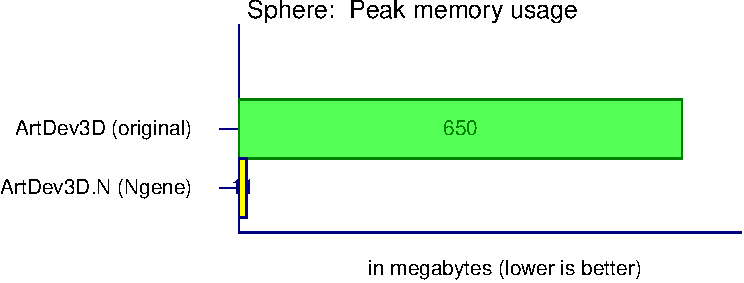
\includegraphics[scale=0.9]{chart_peak-memory-usage}
	\caption{ArtDev3D vs. ArtDev3D.N: Memory usage}
	\label{chart_peak-memory-usage}
\end{figure}

Figure~\ref{chart_peak-memory-usage} shows that ArtDev3D peaks at a staggering 650 MB! The average is only a few MB less. The main culprit for this is Java\texttrademark Virtual Machine. It has been criticized\cite{maio2008} for the garbage collector because of its ridiculous memory consumption. The reason behind is that during allocation and de-allocation, it leaves the memory very fragmented and has a hard time filling the gaps in between, resulting in more memory allocated without being used entirely. Memory usage is important because lowering memory use can also increase overall performance. The computer that these experiments were conducted on has 2 MB of L2 cache. If a program fit into this cache, it would run significantly faster than a program that doesn't. Ngene peaks out at 11 MB but averages at around 7 MB during a run.

	\section{Using the Framework to Study Models}
By now, it has been established that the new framework is able to not only re-implement the models but also reproduce the results. Up to now, we have only seen what is possible technically but has yet to touch the topics that is the true purpose of the framework - the perform studies of development models. Keep in mind that the scope of this thesis does not include a thorough analysis of ADCGP and ArtDev3D. The following chosen topics were picked out to demonstrate what is possible with the framework, without having to worry about interfering factors.


\subsection{Design}
The design of ADCGP is very elegant. It is based on a very simple system of a digital circuit. The cell does not need to do much other than generating input and parsing output. In contrast, ArtDev3D handles much more complex, lower level activities such as protein synthesis and protein requests. It is deeper rooted in biology, a property that is reflected in the original code. On the other hand, it is possible to analyze the inner workings of a cell in ArtDev3D because the control program is rather simple. As the cellular activities are not evolved, it is easier to see what it does because it is of human design. ADCGP lacks this quality because the machine gradually finds out what works in the end. This makes it harder to predict what it is going to do.

With regards to the framework, the design choices of these two models can be easily presented. In this example (fig.~\ref{fig:diagram_ndevframe_msg-comparison}), I've chosen to compare the use of messages in both models. This particular example was chosen because it easily demonstrates the strength of a common platform.

\begin{figure}[!ht]
	\centering
	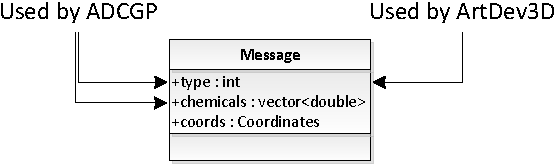
\includegraphics[scale=0.9]{diagram_ndevframe_msg-comparison}
	\caption{ADCGP vs. ArtDev3D: Use of messages}
	\label{fig:diagram_ndevframe_msg-comparison}
\end{figure}

Because the framework enforces use of common yet generic definitions of concepts, we can easily spot their differences. As with the example here, we clearly see that the difference between the two models is the fact that only one model uses chemicals when exchanging information. In fact, that is one of the reasons why chemicals have been reported to complicate things. If everything else had been the same, we could definitely say that this was the cause.


\subsection{Stability}
From the results we've seen so far, there are a number of things that can be said about these models. Most prominently, we see that ArtDev3D is able to evolve perfect specimens within relatively short time. With the sphere experiment, perfect fitness was achieved within just 500 generations. What can't be seen from the results is that it would achieve this typically within 50 generations! In contrast, the ADCGP model requires a lot of generations in order to reach higher fitness. At 10 000 generations, fitness rarely exceeded 0.9. Even when doubling that number, the population was still improving. Obviously, one cannot set it to run forever. The problem seemed to lie in the development method used in the models.

In ArtDev3D, the development or growth would stop after a certain amount of steps regardless of how long the development time. This ensures that the organisms will grow to target shape without overgrowing. H{\o}ye demonstrated this property in his thesis\cite{hoye2006}, and this is reflected by the model's ability to achieve high fitness fast. From the results obtained, it seemed that it is difficult to correctly evolve desired phenotype without knowing how many development steps will be needed. For instance, with the French flag experiment, using four development steps was optimal compared to three or five. Three was obviously not enough because the cells do not have the time to grow properly, while five was too much because the cells started to ``deform''. The new test showed this tendency as well, but it is difficult to state anything for certain with these results. As I've mentioned, one will have to develop a tool to look into each development step to ascertain this behaviour.

	\section{Conclusion}
Ngene Development Framework is a platform for implementing computational development model. It was designed to enable the user to shift its focus from the technical details of implementation to the model itself. The purpose of this framework is to provide a common ground for different models so that any less significant differences are eliminated, making a comparison more accurate as well as easier.

We have seen that it is entirely possible to implement two completely different models using the same code base provided by the framework. As can be seen from the results, the new implementations were able to perform just as well as the original implementations did. We also saw that, with some changes, a model can be made to run more efficiently.

The most important part about being able to port these two models, is that we can clearly see their differences. We can simply put them up side by side, and see, for instance, that ArtDev3D uses only the cell type information of the messages a cell receives. Whereas ADCGP reads both cell types and chemicals. We don't have to worry about minor details, such as the evolutionary algorithms used or the way development was implemented. These are already provided by the framework. The models need only use them.


\subsection{Further Work}

Regretfully, more experiments could have been conducted in order to perform a more thorough comparison between ArtDev3D and ADCGP. It could be interesting to see what the chemicals' real role is. What would happen if chemicals were not used in ADCGP? These are only some of the issues that can be investigated on this platform. It would also have been beneficial to the framework to implement a third model. With only two models, the framework may have easily been ``tailored'' to just these. As more models use the framework, it will become more apparent which parts aren't generic enough for future models. As the purpose of this framework is to be able to compare different models, it is quite essential that it is able to provide for any model. It shouldn't be constricted to just a handful of models.

\subsubsection{Improvements to Ngene and the Development Framework}
\label{sec:improvements}
There are some aspects of the core engine that I would have changed or improved but did not have the time to do so. These changes will further enhance the framework, both in performance and flexibility.

\begin{itemize}
	\item\textbf{Development analysis tool}

	An analysis tool should be able to automatically gather information regarding models implemented within the framework. It should be able to present to the user information such as which properties of the cell are actively changed, or which parts of a message are used. This information should be presented in such a manner that it is easy to compare it side-by-side with another model. In the experiments conducted with ADCGP, it was difficult to tell if the model was suffering from instability or not. This analysis tool should also be able to aid future investigations by enabling the user to walk through and analyze each development step.

	\item\textbf{Further optimizations}
		\begin{itemize}
			\item Currently, the messages are gathered by looping through the cells and finding out what their neighbours are. This is a $O(n^{2})$ algorithm and can be much improved. One way of doing it is to take a snapshot of the organism and pass that object to the cells. The benefit of doing it this way is that it is fast (in the order of $O(n)$) and it also opens up the possibility to simulate chemical diffusion across more cells than the immediate neighbours of a cell.

			\item The use of \texttt{<map>} comes with a penalty as mentioned in chapter~\ref{tbl:speed}. A three-dimensional implementation of a \texttt{<vector>} should be considered as it would give constant lookup and insertion as opposed to $O(log~n)$. It will also remove the need to search for neighbours, as these can be accessed directly given a cell's coordinates.

			\item The Mersenne twister is often criticized for not being very elegant. There has been suggestions that point to other implementations of a pseudo-random number generator that outperform the Mersenne twister while maintaining equal or better quality of randomness. There is also a new implementation of Mersenne twister that should be considered. It is much faster and makes use of SIMD instructions in recent CPUs. Improvements have also been done to increase its quality of randomness Genetic algorithms in general are very dependent on a good random number generator, and having a fast one is only beneficial to the whole engine.

			\item Ngene has implemented OpenMP\footnote{http://www.openmp.org/} in order to utilize multi-core CPUs. This feature was, however, disabled because the framework is not thread-safe. As multi-core CPUs are becoming more common, the framework should be able to utilize such facilities.
		\end{itemize}

	\item\textbf{Making the core interchangeable}

	The genetic algorithm itself should be implemented as a separate module, making it possible to change algorithm depending on the experiments conducted.

	\item\textbf{Ability to swap modules mid-experiment}

	The possibility to swap modules based on circumstances in a population, for instance, half way through an evolution or when the population is converging may produce interesting results. This can be used to simulate genetic drift or other natural phenomena.
\end{itemize}

	\bibliographystyle{ieeetr}
	\bibliography{Bibliography}
	\appendix

\section{Implementing an Ngene Module}
This section will describe the technical details required to implement modules for Ngene. If you've downloaded the source code, the folder structure should be like this (unless it's been changed):

\begin{verbatimtab}
ngene/
 + bin/
 + build/
 + doc/
 + libs/
 + modules/
 + src/
   + Development/
   + Interfaces/
\end{verbatimtab}

\noindent The Interfaces folder contains all the header files that must be included with some modules. These are specified in corresponding modules. For every module, there is one common function that they all must implement.

\begin{verbatim}
/// Sets up the module and makes sure it is ready for use. Every module is
/// initiated this way.
/// \param parameters  The parameters needed to correctly set up the module
void initiate(const char *parameters);
\end{verbatim}

\noindent\texttt{initiate} is called when your module is loaded. This is where the module will recieve its parameters and everything is set up so that it can be used later on. In addition to this, the following sections will describe the rest of the functions that must be implemented in order to be compatible with Ngene.

\subsection{Fitness}

All fitness modules must include the header (path may vary depending on where you installed it):

\begin{verbatim}
#include <Interfaces/Fitness.h>
\end{verbatim}

\noindent The following functions must be implemented.

\begin{verbatim}
/// Assess an individual. The genotype is extracted through
/// individual.genotype, and the fitness is given to individual.fitness.
/// \param[in,out] individual  The individual to assess
void assess(Specimen &individual);

/// Returns the name of this module.
const char *name();
\end{verbatim}

\noindent \texttt{assess()} is called when assessing an individual. The genotype can be extracted from \texttt{individual}. It is an array with generic objects and must be cast into the type that is used. For instance, if your genotype consists of integers, it must be cast into the appropriate data type:

\begin{verbatimtab}
std::vector<int> my_genotype;

for (int i = 0; i < individual.genotype.size(); i++)
{
	// Cast a gene to an integer
	int gene = *boost::unsafe_any_cast<int>(individual.genotype[i]);

	// Store the integer in my own array for later use
	my_genotype.push_back(gene);
}
\end{verbatimtab}

\noindent This does not apply to fitness modules alone, but every module that wishes to make use of the genotype. Once the fitness is calculated, it should be stored in the individual like so:

\begin{verbatim}
individual.fitness = points;
\end{verbatim}

\noindent The individual is now assessed.


\subsection{Genotype}

All genotype modules must include the header (path may vary depending on where you installed it):

\begin{verbatim}
#include <Interfaces/Genotype.h>
\end{verbatim}

\noindent The following functions must be implemented.

\begin{verbatim}
/// Returns the phenotype of given genotype.
/// \param[out]	phenotype  The phenotype returned
/// \param		genotype   The genotype of the wanted phenotype
void phenotype(boost::any &phenotype, const Genotype &genotype);

/// Generates a random genotype.
/// \param[out] genotype  The newly generated genotype
void seed(std::vector<boost::any> &genotype);

/// Return the name of the species, ex. "Traveling salesman problem".
const char *species();

/// Returns the output of a genotype in desired file format.
const char *str(const std::vector<boost::any> &genotype);
\end{verbatim}

\noindent A random genotype is requested when \texttt{seed} is called. This genotype is stored in the container that is provided with the call as parameter.

\texttt{phenotype} is used by the fitness module as it does not necessarily know how to develop an organism. This function receives two parameters. The phenotype can be returned in the first parameter. The second parameter is the genotype itself.


\subsection{Mating}

All mating modules must include the header (path may vary depending on where you installed it):

\begin{verbatim}
#include <Interfaces/Mating.h>
\end{verbatim}

\noindent The following functions must be implemented.

\begin{verbatim}
/// Crosses over two individuals and produces offspring.
/// \param[out] children  The child(ren) produced
/// \param parentA        The first individual of the cross over process
/// \param parentB        The other individual of the cross over process
void mate(std::vector<Specimen> &children, const Specimen &parentA, const Specimen &parentB);

/// Returns the name of this module.
const char *name();

/// Returns the number of offspring this module/method produces
const int offspring();
\end{verbatim}

\noindent\texttt{mate} crosses parentA's genotype with parentB's. The offspring produced are to be stored in \texttt{children}.


\subsection{Mutator}

All mutator modules must include the header (path may vary depending on where you installed it):

\begin{verbatim}
#include <Interfaces/Mutator.h>
\end{verbatim}

\noindent The following functions must be implemented.

\begin{verbatim}
/// Mutates given genotype.
/// \param[in,out] genotype  The genotype to mutate
void mutate(Genotype &genotype);

/// Returns the name of this module.
const char *name();
\end{verbatim}


\subsection{Selector}

All selector modules must include the header (path may vary depending on where you installed it):

\begin{verbatim}
#include <Interfaces/Selector.h>
\end{verbatim}

\noindent The following functions must be implemented.

\begin{verbatim}
/// Randomly selects an individual from a population.
/// \param[out] champ  The selected individual
/// \param candidates  The population to perform selection over
/// \param generation  The current generation
void gene\_select(Population::iterator &champ, Population &candidates, int generation);

/// Returns the name of this module.
const char *name();
\end{verbatim}

\noindent\texttt{gene\_select} performs a random selection, picking out a single individual. This individual is stored in \texttt{champ}.

\end{document}
